\documentclass[12pt]{article}

\usepackage{setspace}
\usepackage{caption}
\usepackage{subcaption}
\usepackage{float}
\usepackage{makecell}
\usepackage{amsmath}
\usepackage{graphicx}
\graphicspath{ {./images/} }
\usepackage[utf8]{inputenc}
\usepackage[russian]{babel}
\usepackage{geometry}
 \geometry{
 a4paper,
 left=20mm,
 right=20mm,
 top=20mm,
 bot=20mm,
 }

\begin{document}

\begin{titlepage}
\begin{center}
    НАЦИОНАЛЬНЫЙ ИССЛЕДОВАТЕЛЬСКИЙ УНИВЕРСИТЕТ ИТМО \\
    Факультет систем управления и робототехники \\
    \vspace*{10\baselineskip}
    {\LARGEЭлектротехника} \\
    \ \\
    \ \\
    \begin{spacing}{1.5}
    {\large Лабораторная работа №1 \\
    ИССЛЕДОВАНИЕ ВНЕШНЕЙ ХАРАКТЕРИСТИКИ \\ ИСТОЧНИКА ЭДС \\
    \ \\
    Вариант 3R382}
    \end{spacing} \\
    \ \\
    \vspace*{10\baselineskip}
    \hfill {Студент: Кирбаба Д.Д.\ \ \ \ \ \ \ \ \ } \\
    \hfill {Группа: R3338\ \ \ \ \ \ \ \ \ \ \ \ \ \ \ \ \ \ \ \ \ } \\
    \hfill {Преподаватель: Китаев Ю.В.} \\
    \mbox{}
    \vfill {г. Санкт-Петербург\\2023}
\end{center}
\end{titlepage}

\subsubsection*{Цель работы}
Исследование режимов работы и экспериментальное определение параметров схемы замещения источника электрической энергии.

\subsubsection*{Ход работы}
Исходные данные:
\[
    r = 5 \ Ohm, \ E = 19 \ V.
\]

\begin{figure}[H]
    \centering
    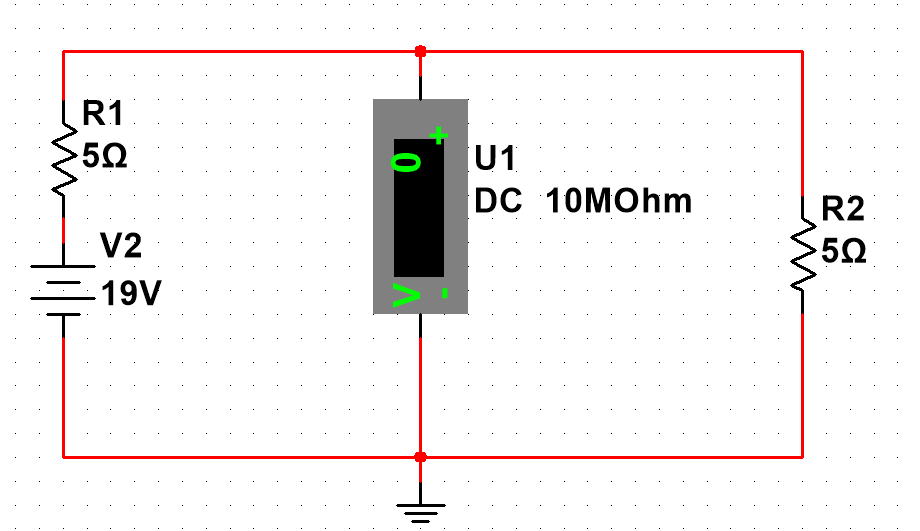
\includegraphics[width=0.5\textwidth]{1_scheme.png}
    \caption{Электрическая цепь.}
    \label{fig:1_scheme}
\end{figure}

Напряжение холостого хода:
\[
    U_{xx} = 19 \ V.
\]

Подберем такое сопротивление нагрузки, чтобы напряжение на нем было равно $\frac{U_{xx}}{2}$:
\[
    r_{xx} = r = 5 \ Ohm.
\]

Проведем измерения напряжений на нагрузке при заданных значений сопротивлений, а также рассчитаем необходимые значения:
\begin{figure}[H]
    \centering
    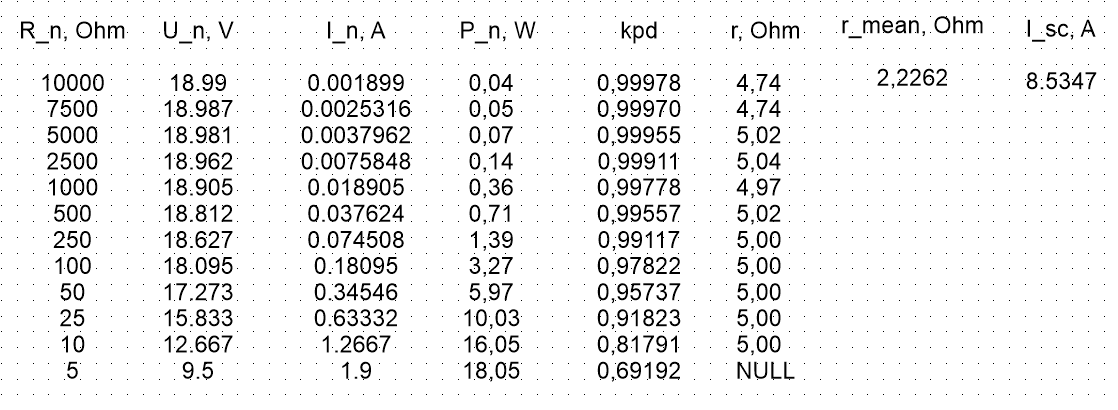
\includegraphics[width=0.7\textwidth]{calcs.png}
    \caption{Расчетная таблица.}
    \label{fig:calcs}
\end{figure}

При высоких значениях $R_{n}$ вычисленные значения внутреннего сопротивления $r$ сильно отличаются от истинного внутреннего значения сопротивления ($5 \ Ohm$) из-за того, что при больших значениях сопротивления на нагрузке ток через нагрузку почти не проходит, следовательно большим изменениям сопротивления соответствуют мизерные изменения тока и напряжения и по этой причине вычисленные значения внутренного споротивления сильно разятся от истинного. \\
Далее, при меньших сопротивлениях на нагрузке, мы наблюдаем существенные различия тока и напряжения вычисленное значение внутреннего сопротивления хорошо совпадает с истинным.

\begin{figure}[H]
    \centering
    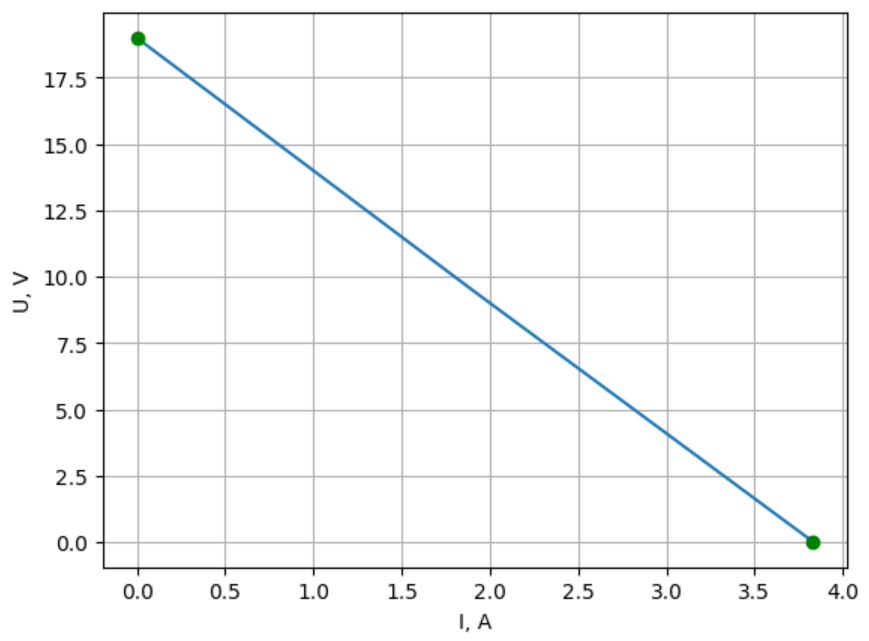
\includegraphics[width=\textwidth]{u_i.png}
    \caption{Внешняя расчетная характеристика.}
    \label{fig:u_i}
\end{figure}

\begin{figure}[H]
    \centering
    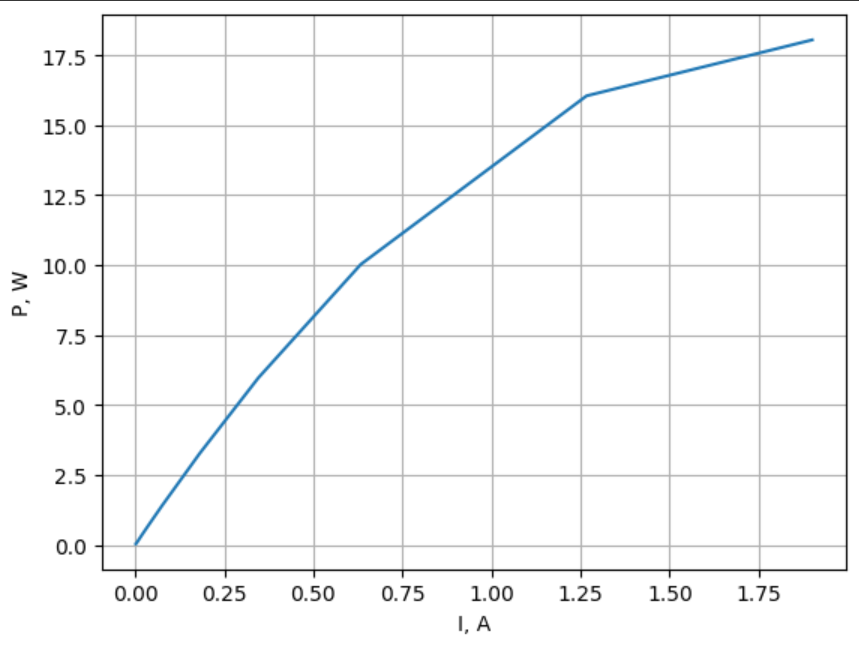
\includegraphics[width=\textwidth]{p_i.png}
    \caption{Зависимость $P(I)$.}
    \label{fig:p_i}
\end{figure}

\begin{figure}[H]
    \centering
    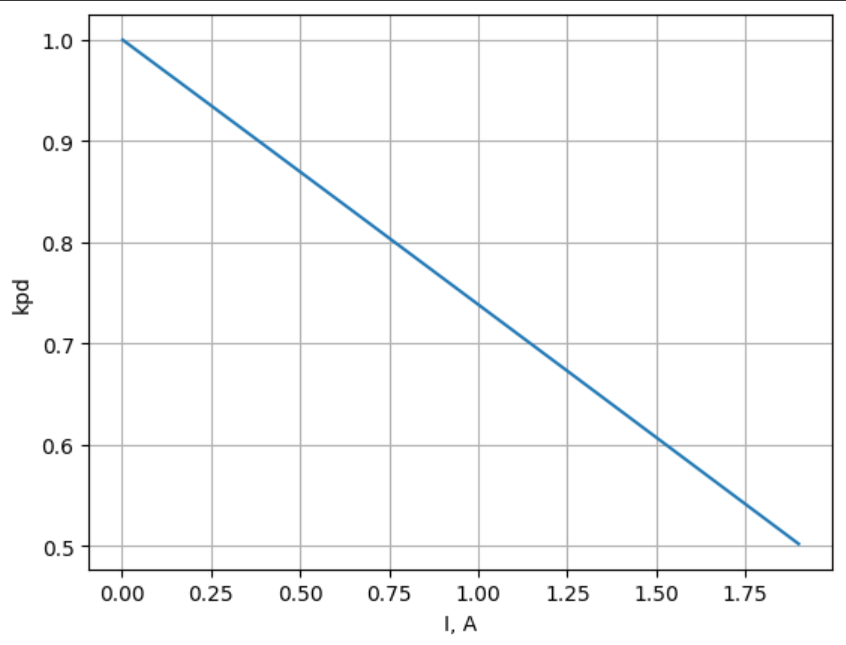
\includegraphics[width=\textwidth]{kpd_i.png}
    \caption{Зависимость $\mu(I)$.}
    \label{fig:kpd_i}
\end{figure}

\subsubsection*{Выводы}
В данной работе были исследованы зависимости тока и напряжения от сопротивления нагрузки. А также были проведены расчеты параметров схемы замещения источника по экспериментальным данным.\\
В конце были построены графики $U(I), \ P(I), \mu(I)$, вид которых подтверждает теоритические зависимости между данными величинами.

\end{document}